\documentclass[journal,12pt,twocolumn]{IEEEtran}

\usepackage{setspace}
\usepackage{gensymb}
\singlespacing
\usepackage[cmex10]{amsmath}

\usepackage{amsthm}

\usepackage{mathrsfs}
\usepackage{txfonts}
\usepackage{stfloats}
\usepackage{bm}
\usepackage{cite}
\usepackage{cases}
\usepackage{subfig}

\usepackage{longtable}
\usepackage{multirow}

\usepackage{enumitem}
\usepackage{mathtools}
\usepackage{steinmetz}
\usepackage{tikz}
\usepackage{circuitikz}
\usepackage{verbatim}
\usepackage{tfrupee}
\usepackage[breaklinks=true]{hyperref}
\usepackage{graphicx}
\usepackage{tkz-euclide}

\usetikzlibrary{calc,math}
\usepackage{listings}
    \usepackage{color}                                            %%
    \usepackage{array}                                            %%
    \usepackage{longtable}                                        %%
    \usepackage{calc}                                             %%
    \usepackage{multirow}                                         %%
    \usepackage{hhline}                                           %%
    \usepackage{ifthen}                                           %%
    \usepackage{lscape}     
\usepackage{multicol}
\usepackage{chngcntr}

\DeclareMathOperator*{\Res}{Res}

\renewcommand\thesection{\arabic{section}}
\renewcommand\thesubsection{\thesection.\arabic{subsection}}
\renewcommand\thesubsubsection{\thesubsection.\arabic{subsubsection}}

\renewcommand\thesectiondis{\arabic{section}}
\renewcommand\thesubsectiondis{\thesectiondis.\arabic{subsection}}
\renewcommand\thesubsubsectiondis{\thesubsectiondis.\arabic{sub subsection}}


\hyphenation{optical networks semiconduc-tor}
\def\inputGnumericTable{}                                 %%

\lstset{
%language=C,
frame=single, 
breaklines=true,
columns=fullflexible
}
\date{March 2021}

\begin{document}

\newcommand{\BEQA}{\begin{eqnarray}}
\newcommand{\EEQA}{\end{eqnarray}}
\newcommand{\define}{\stackrel{\triangle}{=}}
\bibliographystyle{IEEEtran}
\raggedbottom
\setlength{\parindent}{0pt}
\providecommand{\mbf}{\mathbf}
\providecommand{\pr}[1]{\ensuremath{\Pr\left(#1\right)}}
\providecommand{\qfunc}[1]{\ensuremath{Q\left(#1\right)}}
\providecommand{\fn}[1]{\ensuremath{f\left(#1\right)}}
\providecommand{\e}[1]{\ensuremath{E\left(#1\right)}}
\providecommand{\sbrak}[1]{\ensuremath{{}\left[#1\right]}}
\providecommand{\lsbrak}[1]{\ensuremath{{}\left[#1\right.}}
\providecommand{\rsbrak}[1]{\ensuremath{{}\left.#1\right]}}
\providecommand{\brak}[1]{\ensuremath{\left(#1\right)}}
\providecommand{\lbrak}[1]{\ensuremath{\left(#1\right.}}
\providecommand{\rbrak}[1]{\ensuremath{\left.#1\right)}}
\providecommand{\cbrak}[1]{\ensuremath{\left\{#1\right\}}}
\providecommand{\lcbrak}[1]{\ensuremath{\left\{#1\right.}}
\providecommand{\rcbrak}[1]{\ensuremath{\left.#1\right\}}}
\theoremstyle{remark}
\newtheorem{rem}{Remark}
\newcommand{\sgn}{\mathop{\mathrm{sgn}}}
\providecommand{\abs}[1]{\vert#1\vert}
\providecommand{\res}[1]{\Res\displaylimits_{#1}} 
\providecommand{\norm}[1]{\lVert#1\rVert}
%\providecommand{\norm}[1]{\lVert#1\rVert}
\providecommand{\mtx}[1]{\mathbf{#1}}
\providecommand{\mean}[1]{E[ #1 ]}
\providecommand{\fourier}{\overset{\mathcal{F}}{ \rightleftharpoons}}
%\providecommand{\hilbert}{\overset{\mathcal{H}}{ \rightleftharpoons}}
\providecommand{\system}{\overset{\mathcal{H}}{ \longleftrightarrow}}
	%\newcommand{\solution}[2]{\textbf{Solution:}{#1}}
\newcommand{\solution}{\noindent \textbf{Solution: }}
\newcommand{\cosec}{\,\text{cosec}\,}
\providecommand{\dec}[2]{\ensuremath{\overset{#1}{\underset{#2}{\gtrless}}}}
\newcommand{\myvec}[1]{\ensuremath{\begin{pmatrix}#1\end{pmatrix}}}
\newcommand{\mydet}[1]{\ensuremath{\begin{vmatrix}#1\end{vmatrix}}}
\numberwithin{equation}{subsection}
\makeatletter
\vspace{3cm}
\title{ASSIGNMENT 4}
\author{MANIKANTA VALLEPU - AI20BTECH11014}
\maketitle
\newpage
\bigskip
\renewcommand{\thetable}{\theenumi}
Download all python codes from 
\begin{lstlisting}
https://github.com/manik2255/AI1103-PROBABILITY-AND-RANDOM-VARIABLES/blob/main/ASSIGNMENT_4/assignment_4.py
\end{lstlisting}
%
and latex-tikz codes from 
%
\begin{lstlisting}
https://github.com/manik2255/AI1103-PROBABILITY-AND-RANDOM-VARIABLES/blob/main/ASSIGNMENT_4/ASSIGNMENT_4.tex
\end{lstlisting}
\section{GATE 2017 MA PROBLEM.49}
Let X and Y be independent and identically distributed random variables with probability density function
$\fn{x}= \begin{cases}
       e^{-x}  & x>0\\
        0 & otherwise\\
    \end{cases}$
  Then $\pr{max(X,Y)<2}$ equals  
  \section{solution}
Given,
\begin{align}
\fn{x} = 
    \begin{cases}
       e^{-x}  & x>0\\
        0 & otherwise\\
   \end{cases} \label{a}
\end{align}
We know,
\begin{align}
\pr{X<x} = \int_{0}^{x}{\fn{x}}\,dx \label{b}
\end{align}
Using \eqref{a} in \eqref{b},
\begin{align}
\pr{X<x} = \int_{0}^{x}{e^{-x}}\,dx \label{c}
\end{align}
Finding the probability using uniform distribution,Let $F_X(x)$ be the cumulative distribution function of random variable X.
\begin{align}
F_X(x) =\int_{0}^{x}{\fn{x}}\,dx
\end{align}
$F_X(x)$ can be obtained from the uniform distribution of a random variable U on (0,1) and let $U=e^{-x}$.
\begin{align}
0 < U < 1 
\end{align}
As for random variable X also,
\begin{align}
0 < F_X(x) < 1 
\end{align}
This similarity between U and $F_X(x)$ is used to generate the random variable X from U.
\begin{align}
F_X(x) &= \pr{X < x} \\
&= \pr{-log_e U < x}\\
&= \pr{U>e^{-x}}\\
&= 1-\pr{U<e^{-x}}\\
 &= 1- F_U(e^{-x})\label{h}
\end{align}
From uniform distribution,
\begin{align}
F_U(x)=x,0<x<1 \label{i}
\end{align}
\begin{figure}[ht]
    \centering
    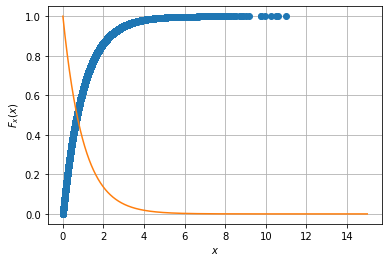
\includegraphics[width=\columnwidth]{assign_4.png}
    \caption{CDF  of random variable X}
\label{fig_1}
\end{figure}
In the figure \ref{fig_1},orange colour graph represents the pdf of the random variable X and blue colour graph represents the cdf of the random variable. 
Using \eqref{h} in \eqref{i}, Cumulative distribution function (CDF) of random variable X is,
\begin{align}
F_X(x) &= \pr{X < x} \\
&= 1-e^{-x} \label{j}
\end{align}
We need to find $\pr{ max(X,Y)<2}$,which is also can be written as
\begin{align}
   \pr{max(X,Y)<2} &=\pr{X<2 ,Y<2}
\end{align}
As X and Y be independent random variables,
\begin{align}
   \pr{max(X,Y)<2} &=\pr{X<2}\pr{Y<2} 
\end{align}
using \eqref{j},
\begin{align}
\pr{max(X,Y)<2} &=(1-e^{-2})(1-e^{-2})\\
&=(1-e^{-2})^{2}\\
&=0.748.
\end{align}

\end{document}
